\chapter{Transformations}
\section{Fourier Transform in Digital Signal Processing}\label{appendix:FT_in_DSP}

In Digital Signal Processing the signal is regarded as a discrete stream of amplitudes in the
time domain. The Fourier Transform is used to transform the signal from the time domain 
to the frequency domain where filters which are hard to implement in the time domain are
more easly implemented.

\begin{figure}[H]
    \centering
    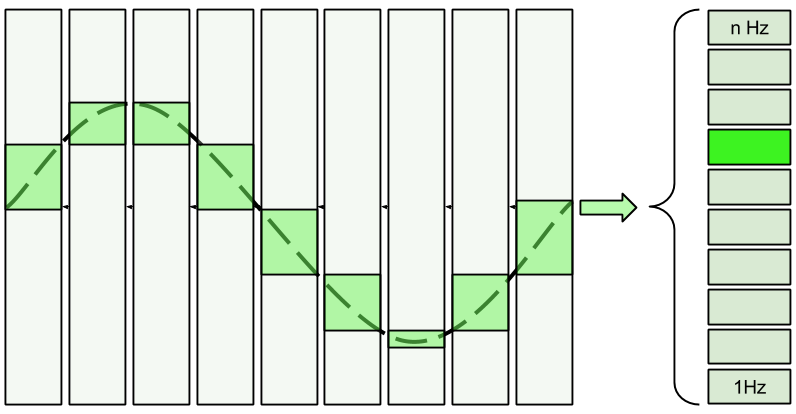
\includegraphics[height=150px]{figures/theory/ft_conceptual}
    \caption{Concept behind the Fourier Transform.}
    \label{fig:ft_conceptual}
\end{figure}
\subsection{Cost efficient implementation of the Fourier Transform}

Cost efficiency is importaint in embedded applications, both in space and time. 
The algorithms mentioned in this appendix are selected based on these criterias.

\subsection{Window size}

The complexity of the algorithm is dependent on the window size. The window size
denotes the number of samples used as input to the algorithm each time it is executed.

\begin{figure}[H]
    \centering
    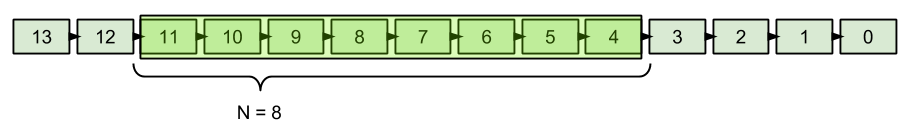
\includegraphics[height=50px]{figures/theory/dft_window}
    \caption{The window consists of the samples included in one calculation of the transform.}
    \label{fig:dft_window}
\end{figure}

The window size is given by equation \ref{eq:window_size}.


\begin{equation} \label{eq:window_size}
window\_size = \frac{samples\_frequency}{frequency\_resolution}	
\end{equation}



\section{Discrete Fourier Transform}\label{appendix:DFT}

The DFT approximates the Fourier Transform for a finite sized window, by assuming the 
input samples are taken from a $n$-periodic function. Due to its complexity, $O(n^2)$, 
it is seldom used in pratice but provides a basis for optimized algorithms. 

%\begin{enumerate}
%\item DFT - Discrete Fourier Transform
%	\begin{itemize}
%		\item FFT - Fast Fourier Transform
%			+ god egnet for 
%			+ godt dokumentert
%			+ tilgjenngelig vhdl IP
%			- kompleks i størrelse og tids
%			- skaper en høyere komplesitet i FPGA cores
%		\item IFFT - Integer Fast Fourier Transform
%			+ unngår fp
%			- dårlig dokumentert
%		\item SDFT - Sliding Discrete Fourier Transform
%			+ enkel å implementer
%			+ godt egnet for strømma applikasjon
%			+ lavere kompleksitet 
%			- potensielt ustabil
%
%			
%	\end{itemize}
%\end{enumerate}


\subsection{Fast Fourier Transform}\label{appendix:FFT}
The Fast Fourier Transform takes a collection of N samples, $x$, as input
and returns the frequencies of this window in time, $X$.
The time complexity of the {\it FFT} is $O(n*log(n))$, therefore the transform is not 
calculated for each new sample input. To avoid discontinuities the transform is performed 
with overlapping windows of the sample stream, and discarding a portion of the output.
The size of $n$ must be a power of 2 for the radix-2 implementation commonly used.

\begin{figure}[H]
    \centering
    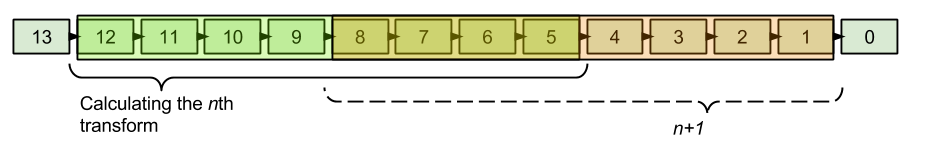
\includegraphics[height=50px]{figures/theory/fft_window_overlap}
    \caption{The illustration shows how the FFT uses overlapping windows to provide a smoother transition. }
    \label{fig:fft_window_overlap}
\end{figure}

\subsection{Integer Fast Fourier Transform} \label{appendix:IntFFT}
The FFT algorithm described above can also be implemented using only integer 
arithmetic. Both the complexity of implementing and executing floating point
arithmetic compared to their interger conterparts makes this a desired property.
The algorithm has the same time complexity as the regular FFT, but the spacial 
complexity increases as the dynamic range of a floating point number is bigger
that that of a integer with the same amount of bits. This means that to get
the same quality a larger word size must be used. The algorithm suggests 
using a lifting structure instead of the butterfly structure used for complex
multiplication.

\subsection{Sliding Discrete Fourier Transform}\label{appendix:SDFT}
The Sliding Discrete Fourier Transform takes one sample, $x_1$, a frequency
domain $X_0$, a historic sample $x_n$ and the fourier coefficients as input.
It returns the frequency domain window, $X_1$ as altered by adding the input
sample, $x_1$ and removing the sample $x_n$. The time complexity of the {\it SDFT}
algorithm is $O(n)$, yet requires that the transform is performed for each 
new sample input. This makes the SDFT well suited for real-time applications.

\begin{figure}[H]
    \centering
    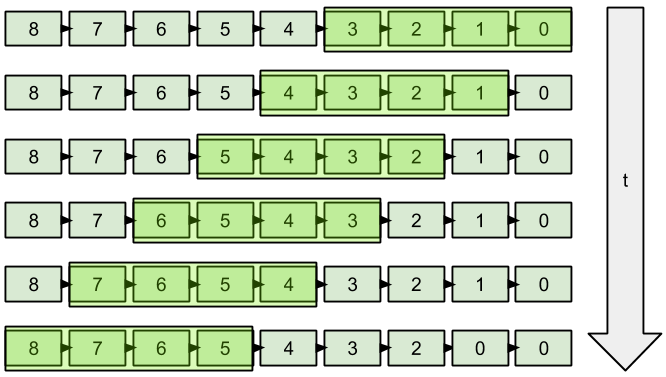
\includegraphics[height=150px]{figures/theory/sdft_window_slide}
    \caption{The SDFT's window slides one sample per time unit.}
    \label{fig:sdft_window_slide}
\end{figure}